\label{sec:fak_sol}
% TODO: plot 5.1 colorbar frequency, cartoon of spots
% TODO: more story telling
In this section, we investigate the conformation of soluted FAK (FAK-SOL) for the \martini{} force field. Since the secondary structure of the two domains is fixed due to the elastic network, the focus is on the FERM-kinase interface.\\
\\
% TODO: swap spot numbering
First, the COM distances of F1 to the N-lobe ($d_\text{F1-N}$) and F2 to the C-lobe ($d_\text{F2-C}$) are considered. The two dimensional histogram of the distances reveals two different states (\autoref{free:f2clf1nl}). Spot 1 refers to conformations, which are partially opened at the F2 - C-lobe interface, but close at the F1 - N-lobe interface. In contrast to this, the conformations of spot 2 refers to states in which F2 and the C-lobe gets closer while the distance between F1 and the N-lobe is increased. The corresponding 3D structures are shown in \autoref{free:3d}. They induce that spot 1 refers to a configuration in which the kinase is slightly tilted against the FERM domain while it is in line for configurations associated with spot 2. We observed several transitions between the spots during the simulation, which indicates a sufficiently long simulation time. In total $47.4\%$ of the obtained distances were located in spot 1 and $52.6\%$ in spot 2.\\
However, the transitions only have a minor effect upon the contact area (\autoref{free:ca}).  Spot 2 shows a slightly larger mean value of $27.6\,\si{\nano\metre}^2$ as compared to $27.1\,\si{\nano\metre}^2$ in spot 1.\\
%
%
%
\begin{figure}
	\subcaptionbox{\label{free:f2clf1nl}}[0.49\textwidth]{
		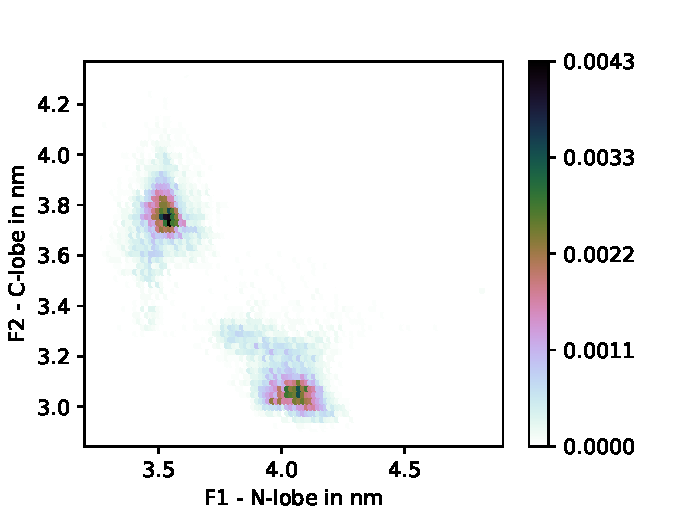
\includegraphics[height=5.2cm]{figures/results/free_f1f2}
	}\hfill%
	\subcaptionbox{\label{free:ca}}[0.49\textwidth]{
		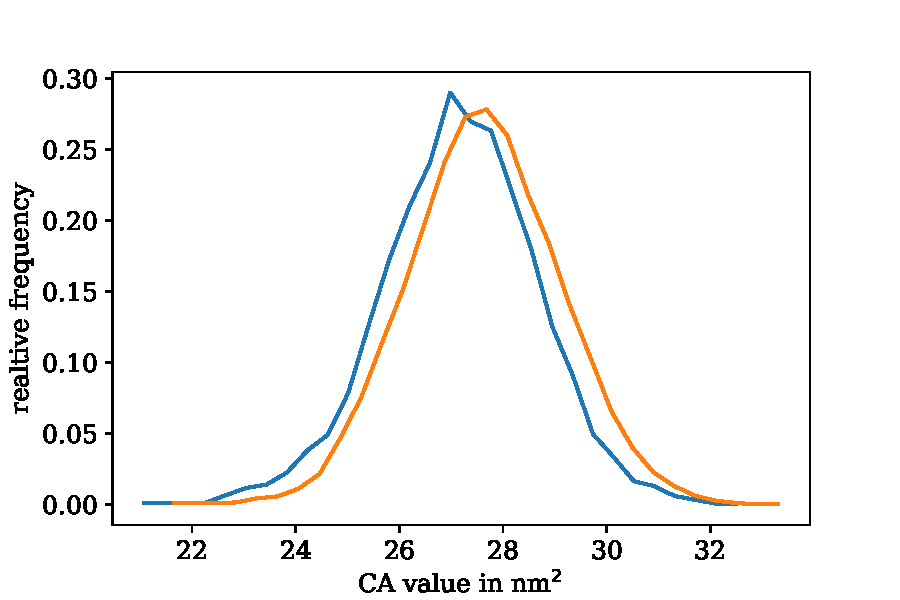
\includegraphics[height=5.2cm]{figures/results/free_ca}
	}%
	\nicecaption{Domain distances and contact area of FAK-SOL}{(\subref{free:f2clf1nl}): two dimensional hexagonal binning plot of $d_\text{F1-N}$ and $d_\text{F2-C}$ which shows the two spots. (\subref{free:ca}): distribution of CA for the two spots.}
\end{figure}
% TODO: label spots
%
%
%
\\
The average contact map of the interface between the FERM domain and the kinase for frames in spot 2 is shown in \autoref{free:contact}. Two regions can be identified. The first one (area 1) is located between F1 and the N-lobe/activation loop. It shows especially contacts between \acid{Y}{576} and \acid{Y}{577} and residues of the FERM domain. The minimal distance in this area, occurring between residue \acid{H}{41} and \acid{Y}{576}, is $0.45\,\si{\nano\metre}$ with an RMSF value of $0.03\,\si{\nano\metre}$. This area reflects the burying of the activity-regulating residues in the closed state (see \autoref{free:3d_spot2}).\\
The second region (area 2) is located between F2 and the C-lobe. The spots occur around the residues \acid{Y}{180} and \acid{D}{200} of F2 as well as \acid{F}{596} and \acid{R}{665} of the C-lobe. The minimal distance in this area occurs between \acid{Y}{180} and \acid{F}{596} with $0.45\,\si{\nano\metre}$ and an RMSF value of $0.02\,\si{\nano\metre}$. Mutation experiments showed these two residues to have an important effect upon the interface \autocite{structFAK}, which fits to these observations.\\
% TODO: add to "area 2" smth like observed in spot 2 only.
The linker shows contacts with both domains. The minimal distances in the marked areas occur between the autophosphorylation site \acid{Y}{397} and \acid{H}{58} of F1 ($0.45\,\si{\nano\metre}$, RMSF $0.03\,\si{\nano\metre}$) as well as \acid{Y}{397} and \acid{Y}{576} of the kinase ($0.50\,\si{\nano\metre}$, RMSF $0.10\,\si{\nano\metre}$). Furthermore, several interactions occur between the residues in the linker itself, namely, between \acid{S}{379} to \acid{V}{389} and \acid{T}{394} to \acid{I}{400} (area 5). Also in this spot, the minimal distance occurs between \acid{Y}{397} and \acid{T}{386} ($0.52\,\si{\nano\metre}$, RMSF $0.04\,\si{\nano\metre}$). The density in this area implies that the linker forms a ball, which is slightly plunged into the interface of the FERM domain and the kinase (regarding area 3 and area 4). This can be seen also in the 3D structure in \autoref{free:3d_spot2}. Our observations support the thesis that autophosphorylation is prevented in the closed conformation by a binding of the linker to the FERM domain \autocite{pap003}.\\
\\
The contact map for configurations of spot 1 shows similar features as obtained for spot 2. However, in area 2 fewer contacts occur (see \autoref{free:contact}), which is reasonable, since the C-lobe is tilted against the FERM domain. % still not clear, why in mutant of Y180 nicht diese pose eingenommen wird.
%
%
\begin{figure}
	\centering
	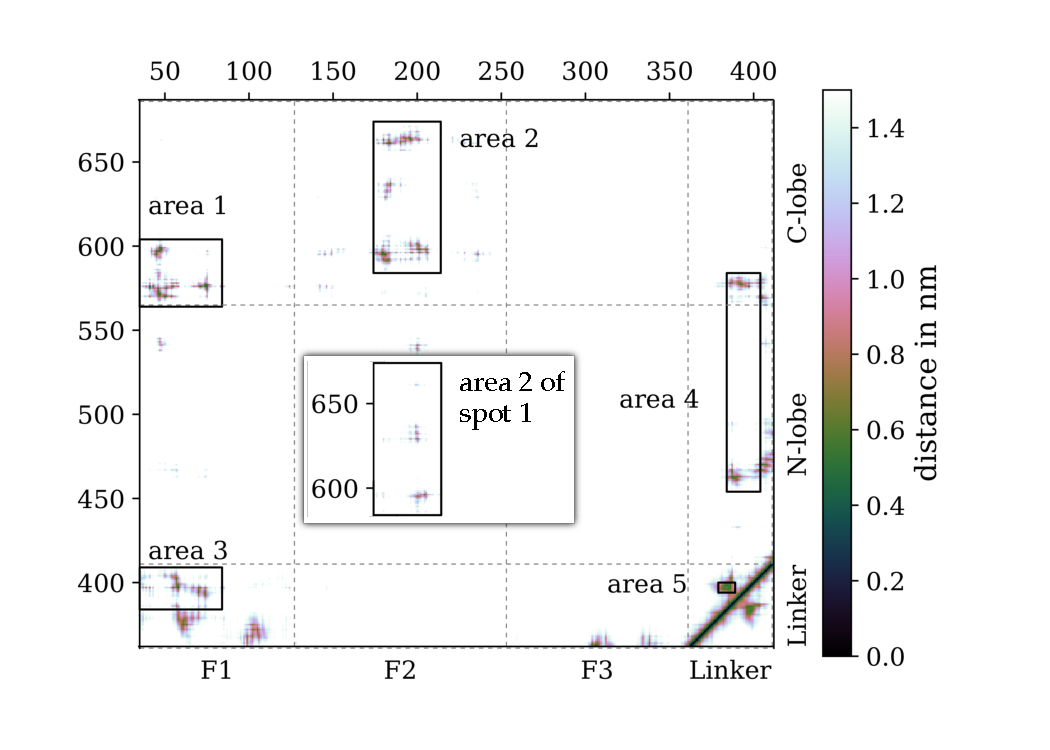
\includegraphics[width=.8\textwidth]{figures/results/contactmap_free_bothspots}
	\nicecaption{Contact map of FAK-SOL}{Contact map of the FERM-kinase interface and the linker region.}
	\label{free:contact}
\end{figure}
% TODO: spot 1 außerhalb von spot 2, besser linken und caption!!
%
%
%
%
%
%
\begin{figure}
	\subcaptionbox{\label{free:3d_spot1}}[0.32\textwidth]{
		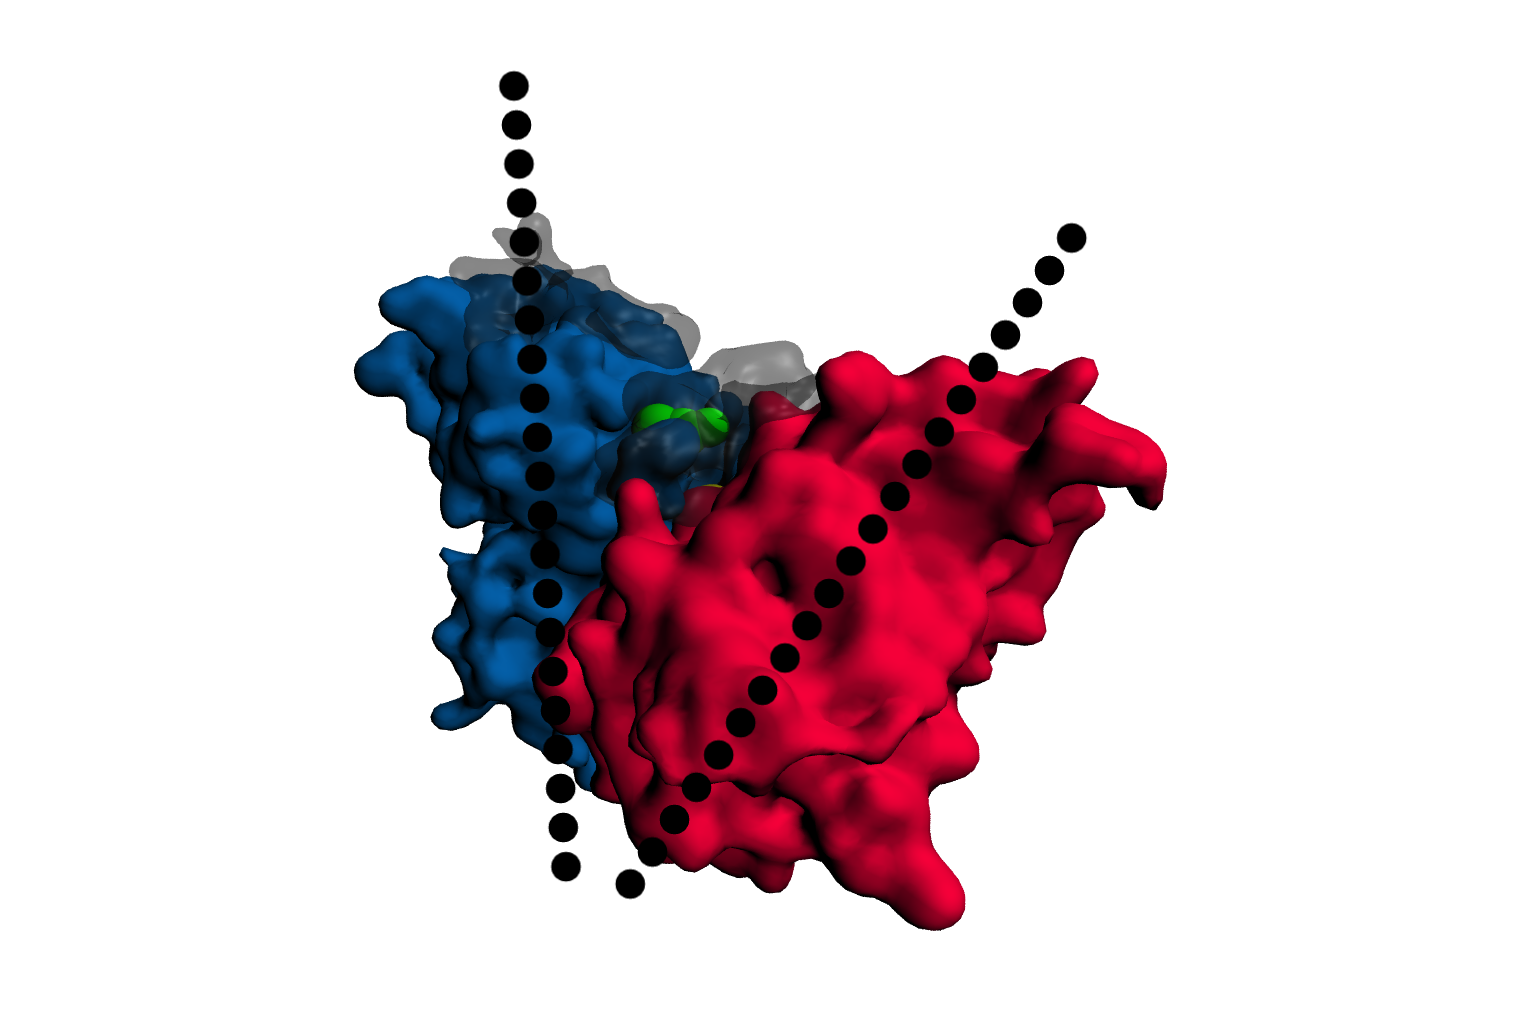
\includegraphics[height=4cm]{figures/results/fak_spot1}
	}\hfill%
	\subcaptionbox{\label{free:3d_spot2}}[0.32\textwidth]{
		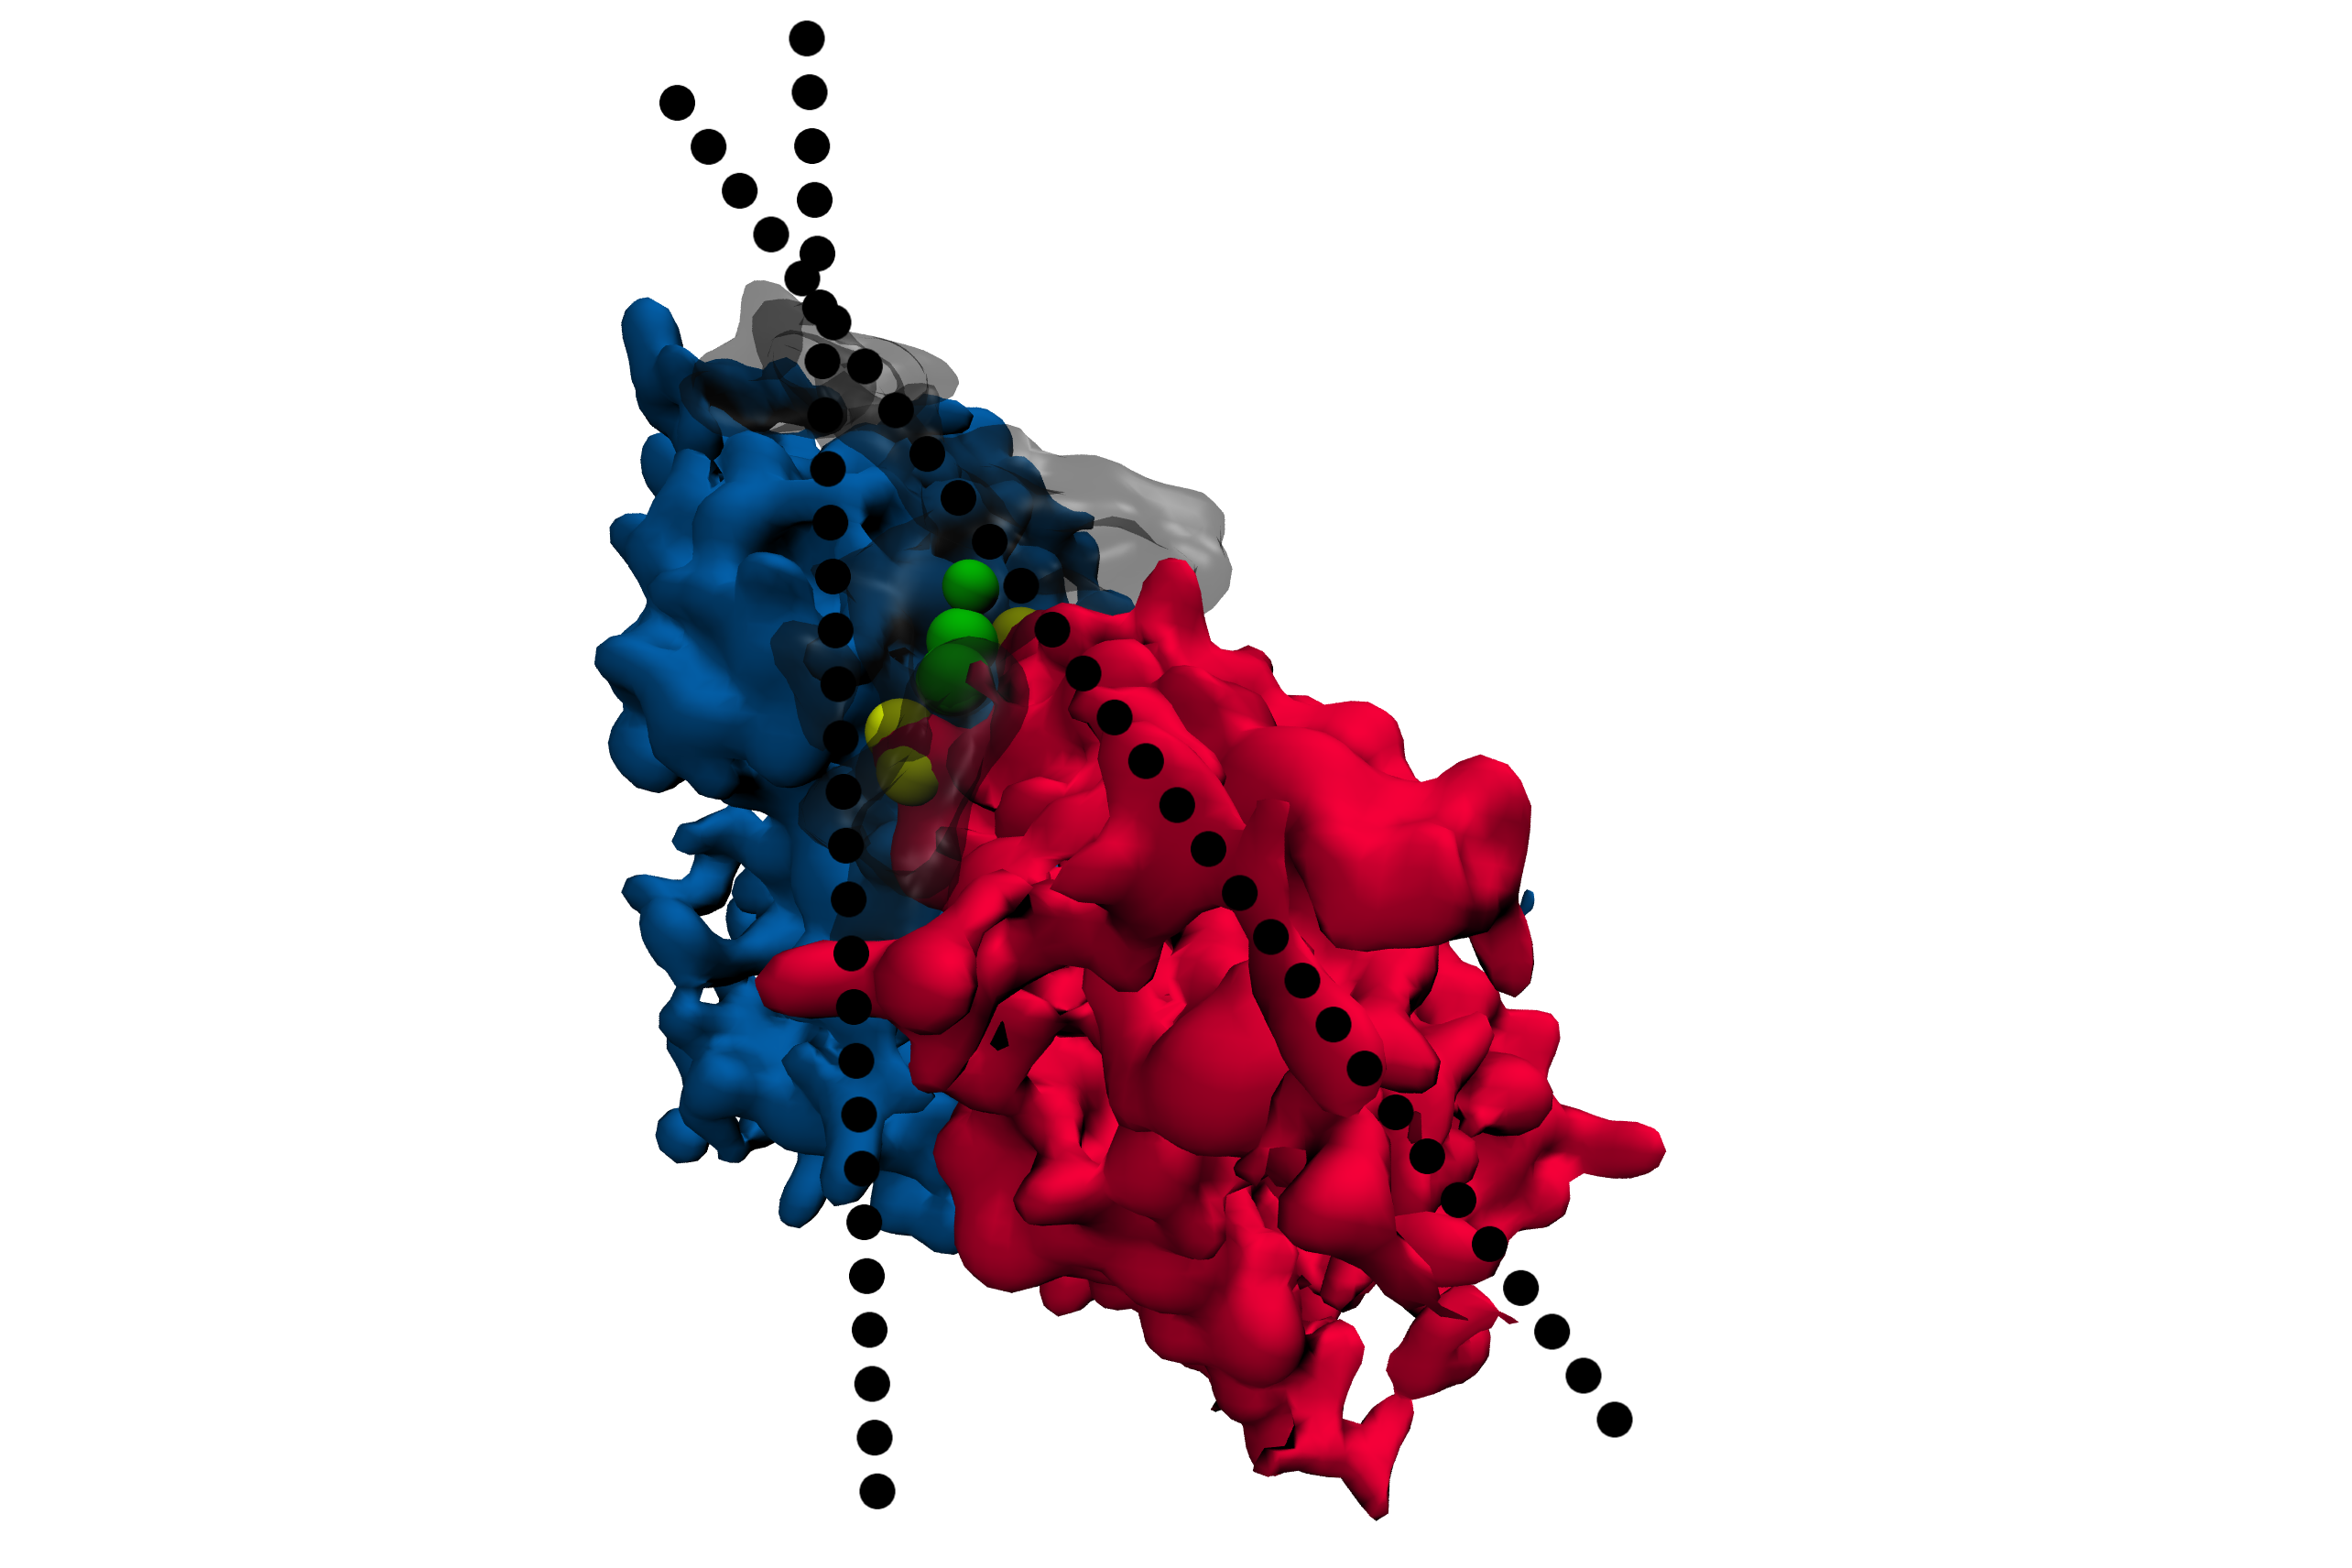
\includegraphics[height=3.5cm]{figures/results/fak_spot2}
	}\hfill%
	\subcaptionbox{\label{free:3d_spot_top}}[0.32\textwidth]{
		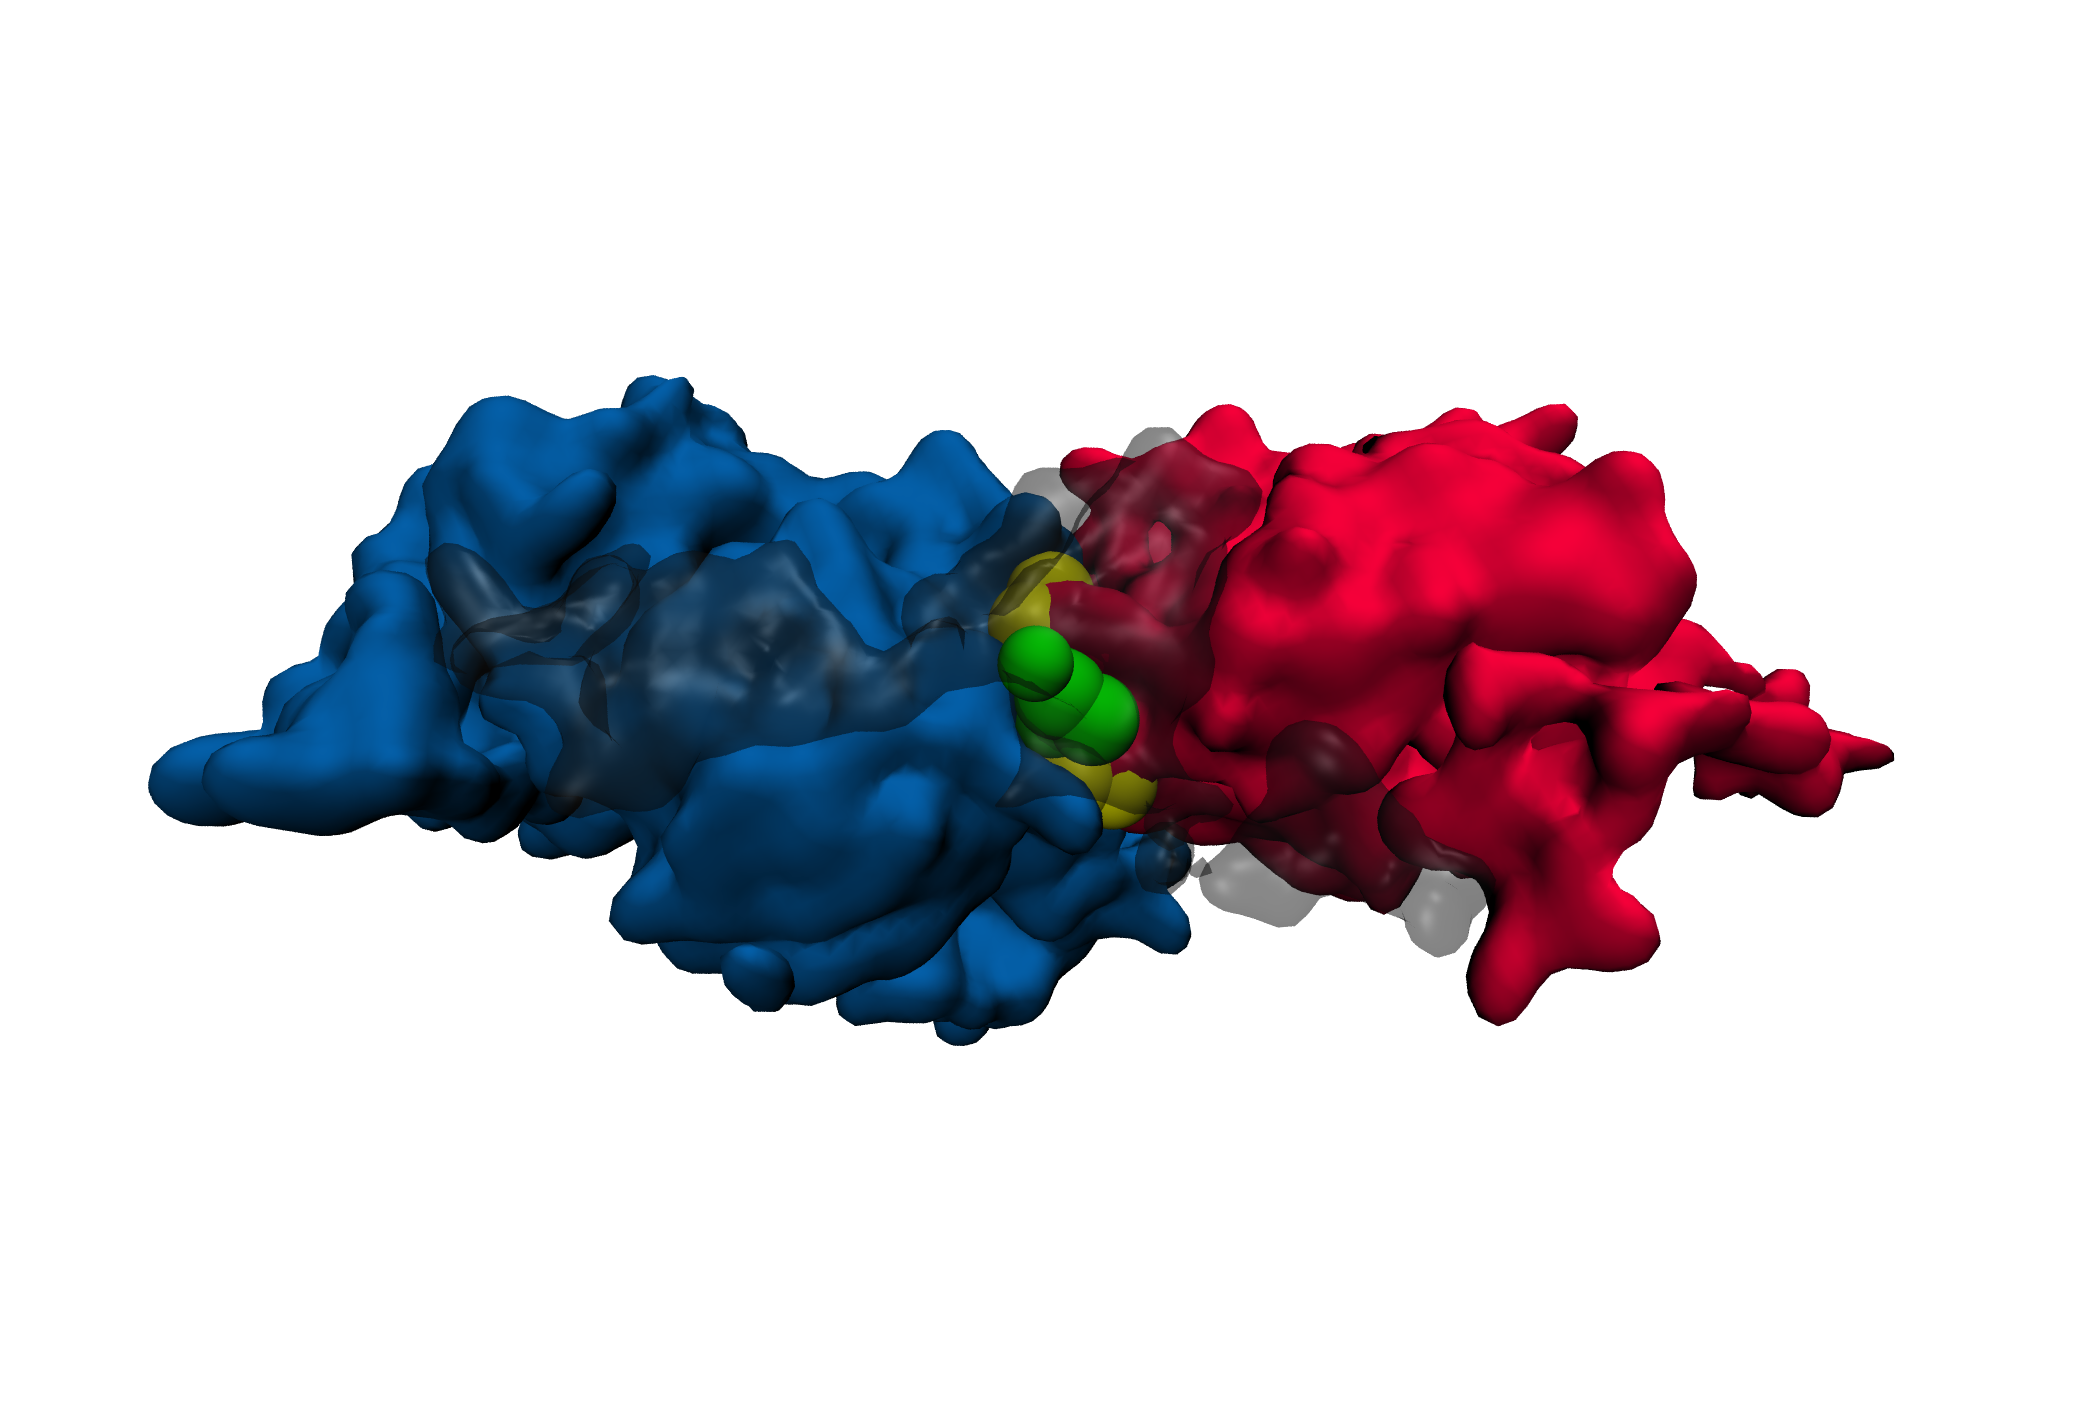
\includegraphics[height=3.5cm]{figures/results/fak_spot2_top}
	}
	\nicecaption{3D structure of the two states in FAK-SOL}{The 3D structures show the FERM domain (blue), the kinase (red) and the linker (black, transparent). The autophosphorylation site \acid{Y}{397} (green) is plunged into the interface and hidden by the linker. \acid{Y}{576} and \acid{Y}{577} (yellow) are shielded by the FERM domain.\\
	(\subref{free:3d_spot1}, spot 1): The kinase is tilted against FERM. (\subref{free:3d_spot2} and \subref{free:3d_spot_top}, spot 2): Both domains are in line.}
\label{free:3d}
\end{figure}
%
%
%
